\setchapterstyle{kao}
\setchapterpreamble[u]{\margintoc}

\chapter{Design and Simulation} % How I thought it was going to work
\labch{tc-design-and-simulation}

\textbf{Disclaimer:} This process was a lot more length and tedious than depicted in the following chapter. It mostly consisted of trial and error, which started with an more or less educated guess and ended in cluelessness and despair. But those errors don't add a lot of value to understanding the topic, so I won't go into much detail.

\section{The Coils}

The goal was to design an air coil with a resonant frequency of 4MHz. This frequency was chosen, since it is high enough to work well with an class E amplifier, but low enough to not run into too many RF related problems. It was also already known to have worked with a few other class E tesla coils.

\subsection{Rough Estimation of the Secondary Coil}

The inductance of a single-layered air solenoid coil can be calculated with

\begin{equation}\label{eq-inductivity}
    L = \mu_0 \frac{N^2 A}{l}
\end{equation}

The parasitic capacitance, depending on its length \(l\) and its diameter \(D\) can be calculated with\sidecite{self-capacitance}

\begin{equation}\label{eq-parasitic-capacitance}
    C_L = \frac{4\varepsilon_0}{\pi} \cdot l \cdot \left( 1 + 0.8249 \frac{D}{l} + 2.329 \left(\frac{D}{l}\right)^{1.5}\right)
\end{equation}

Defining the length to diameter ratio of the coil to be 4, and \(d_w\) to be the diameter of the wire, both formulas can be rewritten to only depend on \(l\) and \(d_w\). 

\begin{equation}
    L = \mu_0 \frac{l^3\ \pi}{32 d_w^2}
\end{equation}

\begin{equation}
    C_L = \frac{4\varepsilon_0}{\pi} \cdot l \cdot 1.49735
\end{equation}

Those equations can then be set into the formula for the resonant frequency of an LC circuit.

\begin{equation}
    f = \frac{1}{2\pi \cdot \sqrt{0.1872 \cdot \dfrac{1}{d_w^2} \cdot \mu_0 \varepsilon_0 \cdot l^4}}
\end{equation}

Rearranging the equation to \(l\)

\begin{equation}
    l = \frac{1}{\sqrt[\scalebox{1}{4}]{4\pi^2 f^2 \cdot0.1872 \cdot \dfrac{1}{d_w^2} \cdot \mu_0 \varepsilon_0}}
\end{equation}

With a frequency of 4MHz and a wire diameter of 0.35mm, the length of the coil turns out to be around 100mm and the diameter therefore around 25mm.

Due to the materials available, a 30 mm tube was used to wind the wire around. By using equation \ref{eq-inductivity} and \ref{eq-parasitic-capacitance}, an equation can be derived, which describes the relationship of all relevant variables.

\begin{equation}
    f = \frac{1}{2\pi \dfrac{D}{d_w} \sqrt{\mu_0 \varepsilon_0 \left( l^2 + 0.8245 D l + 2.329 D^{1.5} \sqrt{l} \right)}}
\end{equation}

Using Wolfram Alpha to solve this equation for \(l\) with a \(D\) of 30 mm gives a length of 112 mm.
% 4000000 = 1/(2π(0.03/0.00035)Sqrt[11.1265e-18*(Power[x,2]+0.8245*0.03*x+2.329*Power[0.03,1.5]*Sqrt[x])]) solve for x

\subsection{Tuning the Secondary Coil}\label{TC-tuningTheSecondary}

Tuning the coil to the correct frequency is essential, because all calculated values from above are highly idealized. For example, equation \ref{eq-parasitic-capacitance} is said to have a standard deviation of \(\sigma_{CL} \text{in pF} = 3.6 \cdot D\), which leads to a standard deviation of around 116 kHz of the resonant frequency of the coil. In addition, the relative permeability and permittivity factor of the carrier material are not taken into consideration in the calculations.

The coil was tuned by exciting the base of the secondary coil with a sinusoidal voltage. An oscilloscope probe, formed into a current loop, was placed near the top of the coil. The closer the excitation frequency was to the resonant frequency of the coil, the higher the measured voltage on the oscilloscope. The frequency, at which the measured voltage was at its maximum, was the resonant frequency of the coil. By adding or removing windings, the resonant frequency could be lowered or raised, until it exactly matched 4MHz\sidenote{In order to avoid adding windings, which is more tedious than removing them, the coil was wound a little longer than calculated}. % Add how close the original calculations were

\subsection{Designing the Primary Coil}
\label{sec:designing-the-primary}

The primary coil offers a lot of design freedom and flexibility, but this also means, that there is no \enquote{correct} or \enquote{ideal} design, but only one, which has been observed to work well. It mostly comes down to optimizing the coupling coefficient between the two coils. If it's too low, not enough energy will be transferred to the secondary, but to raise it, the coils have to be moved closer together which leads to flashover, due to too low insulation. % Test tesla coil with coupling factor of 0.10 to 0.15  Source: book page 55
This limitation can be bypassed by making the primary coil smaller at the bottom, where the voltage is higher and larger at the top, where the voltage is higher. This results in the well-known conical shape known from many tesla coils.

\begin{marginfigure}
\centering
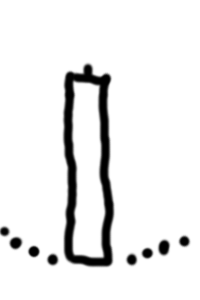
\includegraphics[width=0.6\textwidth]{simon/resources/teslaCoilSketch.png}
\end{marginfigure}

\subsection{Simulating the Coupling Coefficient}

In order to simulate the resonant transformer, its coupling coefficient has to be known. It describes how tightly the two coils are magnetically coupled and how much of the generated magnetic field of one coil is induced in the other. The simulation tool EleFAnT2D\sidenote{\textbf{Ele}ctromagnetic \textbf{F}ield \textbf{An}alyis \textbf{T}ool, developed IGTE, TU Graz} was used to simulate the magnetic flux in the system. The coupling coefficient can be described as

\begin{equation}
    k = \frac{\Phi_{ind}}{\sqrt{\Phi_P \cdot \Phi_S}}
\end{equation}

where \(\Phi_{ind}\) is the flux linkage between the two coils and \(\Phi_P\) and \(\Phi_S\) are the flux of the primary and secondary coil, respectively.\todo{Is it really?} By using this formula and the simulated values, the coupling factor as a function of the vertical displacement of the primary coil has been calculated as can be seen in figure \ref{fig:coupling-factor}.

\begin{figure}[h!]
    \centering
    \begin{tikzpicture}
    \begin{axis}[
    width = 0.9\textwidth,
    minor tick num = 1,
    grid = both,
    ymax = 25,
    xmin = -20,
    xmax = 20,
    xlabel = Vertical displacement in mm,
    ylabel = Coupling factor in \%
    ]
    \addplot+[mark options={black!50}, draw=black] table [x=d, y=k, col sep=comma]{simon/resources/couplingFactor.csv};
    \draw (axis cs:0,-10) -- (axis cs:0,18.397) -- (axis cs:-20,18.397);
    \draw (axis cs:-18,18.9) node(){\(18.4\)};
    \end{axis}
    \end{tikzpicture}
    \caption{Position dependent coupling factor}
    \label{fig:coupling-factor}
\end{figure}

As expected, the coupling factor gets smaller the farther away the primary coil moves from the center of the secondary coil.

\subsection{Modeling the Transformer in LTSpice}

The analog electronic circuit simulator LTSpice, which was used for this project, did unfortunately not provide any tools to simulate the arc breakout at the secondary coil, which is necessary for testing the continuous operation performance. Also, modeling the magnetic coupling of the transformer involved a trick, which is worth mentioning.

\subsubsection{The Magnetic Coupling}

\sidecite{ltspice}

To simulate a transformer in LTSpice, the K directive can be used. For example, \cinl{K L1 L2 0.3} couples the inductivities L1 and L2 with a coupling coefficient of 30\,\%.

\subsubsection{The Arcing}

\begin{marginfigure}[5mm]
    \centering
    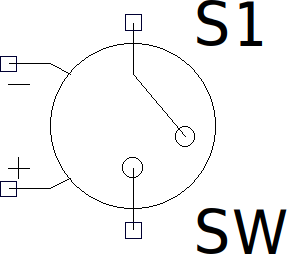
\includegraphics[width=0.5\textwidth]{simon/resources/ltspice_sw.png}
    \caption{Voltage Controlled Switch}
    \label{fig:ltspice_sw}
\end{marginfigure}

When the voltage in the secondary coil \(V_{SC}\) is high enough to ionize the air around it, a spark forms. This spark persists as long as the coil can provide enough current to keep it alive. After \(V_{SC}\) dropped to a very low level, the spark extinguishes and allows the secondary coil to charge up again.

A very basic way to model this behaviour in LTSpice is to use a voltage controlled switch with some conditional logic. A voltage controlled switch is an ideal, lossless component which simply connects or disconnects its two terminals depending on the voltage difference of its \texttt{+} and \texttt{-} pins\sidecite{ltspice}. The switch is connected in parallel to the secondary coil's capacitance, which gets discharged rapidly when the switch closes.

To specify the switch's characteristics, a new switch model has to be defined. For the example of a switch without a hysteresis, this can look like \cinl{.model model_name SW(Vt = 1k)}. This switch is closed above and opened below 1\,kV, and has an \(R_{ON}\) of 1\,\(\Omega\), \(R_{OFF}\) of \(1\,T\Omega\), and no additional parasitics. 

However, it is not possible to use \(V_{SC}\) directly as the control voltage, because it returns to zero two times per period, which would instantly turn off the switch again. Instead the switch should turn off when the current through it falls below a certain threshold. For this a D latch and an \emph{arbitrary behavioural voltage source} can be used\sidecite{spark-gap}. This kind of voltage source can be configured to output an arbitrary voltage based on logical and mathematical expressions. The complete spark gap model can be seen in figure \ref{fig:ltspice-sparkgap}.

\begin{figure}[h!]
    \centering
    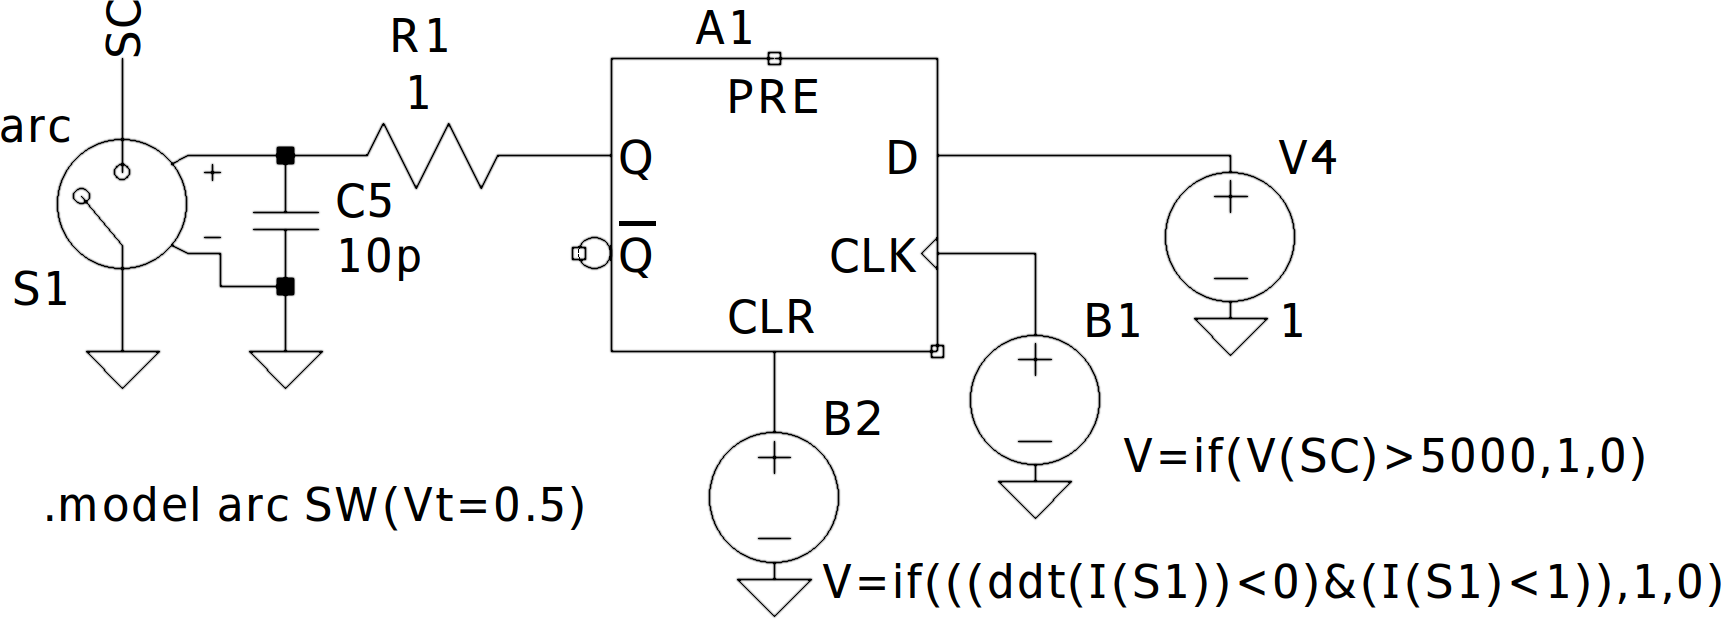
\includegraphics[width=0.9\textwidth]{simon/resources/ltspice_sparkgap.png}
    \caption{Spark Gap Model in LTSpice}
    \label{fig:ltspice-sparkgap}
\end{figure}

\texttt{V4} supplies a constant \texttt{HIGH} signal to the latch's input. \texttt{B1} turns the \texttt{CLK} input \texttt{HIGH} as soon as \(V_{SC}\) reaches \(5\,kV\). And lastly, \texttt{B2} resets the latch if the current falls below \(1\,A\). The \emph{falling} is essential here, because at the moment the switch turns on, the current also is below \(1\,A\), which would turn off the switch again. With the additional \cinl{ddt(I(S1))<0} condition it was made sure that the current has to be decreasing. The low pass filter consisting of \texttt{R1} and \texttt{C5} adds a tiny delay to the latch's output signal, without which LTSpice would not be able to simulate the circuit. Figure \ref{fig:spark-gap-simulation} shows the voltage \(V_{SC}\) after the spark gap has been put into place.

\begin{figure}[h!]
    \centering
    \resizebox{0.9\textwidth}{!}{
    \begin{tikzpicture}
      \begin{axis}[
        y filter/.code=\pgfmathparse{#1 / 1000},
        ylabel = \(V_{SC}\) in \(kV\),
        x filter/.code=\pgfmathparse{#1 * 1000000},
        xlabel = \(t\) in \(\mu s\),
        ytick= {-5,0,5},
        ymajorgrids,
        ]
        \addplot table[x=t,y=v,col sep=comma, mark=none]{simon/resources/sparkgap.csv};
      \end{axis}
    \end{tikzpicture}}
    \caption{Spark Gap Simulation}
    \label{fig:spark-gap-simulation}
\end{figure}

\section{Class-E Design}

As already explained in aaaaa, it is everything but trivial to design a class E amplifier to drive a tesla resonator. However, for the sake of demonstration, the following subsection will go through the design process of a class E amplifier with an ohmic load.

\subsection{The Design Process}

Nathan Sokal, who popularized the class-E amplifier along with Alan Sokal, presented a set of revised design equations in 2001 \sidecite[-3mm]{sokal-qex}. Unlike previously published equations, they include the dependence of the loaded Q factor\sidenote{It describes how damped a resonator is, or in other words, how quickly it dissipates its oscillating energy.} as well as on the output power.

The goal of this amplifier is to create 50\,W of output power in a load of 22\,\(\Omega\) at a frequency of 4\,MHz. The Q factor of the load network has to be chosen by the designer and involves 

\begin{displayquote}
\enquote{a trade-off among the operating bandwidth (wider with lower \(Q_L\)), harmonic content of the output power (\textelp{} lower with higher \(Q_L\)) and power loss in the parasitic resistances of the load-network inductor \(L_2\) and capacitor \(C_2\) (lower with lower \(Q_L\)).}
\end{displayquote}

The chosen value for \(Q_L\) is 5, because it is a common starting value for simple class-E amplifiers. The switching device will be a MOSFET, so the saturation voltage used in the equations have already been set to zero. Also, to make the calculations clearer, all numbers, as well as the results have been rounded to three significant digits. The necessary supply voltage is

\begin{equation*}
    V_{CC} = \sqrt{R \cdot P \cdot 1.73 \cdot \frac{1}{1 - \frac{0.452}{Q_L} - \frac{0.402}{Q_L^2}}} = 46.1\,V\textnormal{\,.}
\end{equation*}

The expected peak drain-source voltage on the MOSFET is 3.56 times the supply voltage plus a safety factor of around 20\%, which means that the MOSFET has to have a drain-source breakdown voltage of at least 197\,V. 

The choke inductance \(L_1\), again, has to be chosen in order to calculate the remaining component values. It has to be big enough to force enough current into \(C_1\) and keep the current ripple low. A rule of thumb is that \(X_{L1}\) should be at least 30 times greater than \(X_{C1}\). However, since \(C_1\) slightly depends on \(L_1\), this is an iterative process. A value for \(L_1\), which turns out to work well is \(130\,\mu H\). \(C_1\), \(C_2\), and \(L_2\) can then be calculated with

\begin{equation*}
    C_1 = \frac{1}{34.2\cdot f R} \cdot \left( 1 + \frac{0.914}{Q_L} - \frac{1.03}{Q_L^2} \right) + \frac{0.6}{(2 \pi f)^2  \cdot L_1} = 387\,pF\textnormal{\,,}
\end{equation*}
\begin{equation*}
    C_2 = \frac{1}{2 \pi  f  R} \cdot \frac{1}{Q_L - 0.105} \cdot \left( 1 + \frac{1.01}{Q_L - 1.79} \right) - \frac{0.2}{(2 \pi f)^2 \cdot L_1} = 482\,pF \textnormal{\,, and}
\end{equation*}
\begin{equation*}
    L_2 = \frac{Q_L \cdot R}{2 \pi f} = 4.38\,\mu H\textnormal{\,.}
\end{equation*}
 
Since \(C_1\) is the sum of the capacitor \(C_{1*}\) and the MOSFET's output capacitance \(C_{1_M}\), % better convention?
this output capacitance cannot be greater than \(C_1\) itself.

Based on the previous calculations, the MOSFET must have

\begin{itemize}
    \item a drain-source breakdown voltage greater than 197\,V,
    \item an output capacitance less than 387\,pF,
    \item switching times much smaller than 125\,ns (\nicefrac{T}{2}), and
    \item a maximum power dissipation of at least 5\,W.
\end{itemize}

One MOSFET which meets all these criteria is the BSC12DN20NS3. It has a drain-source breakdown voltage of 200V, an output capacitance of 39pF, turn-off and turn-on times of less than 5 ns and a maximum power dissipation of 50W. The capacitor \(C_{1*}\) therefore is \(387\,pF - 39\,pF = 348\,pF\).

The driver was then simulated using LTSpice. The Spice model for the BSC12DN20NS3 can be found in QR code \newqrcode{https://www.infineon.com/dgdl/Infineon-PowerMOSFET_OptiMOS_PSpice_200V_N-Channel-SimulationModels-v02_00-EN.zip?fileId=5546d4624f72be57014f73c9c774060e}{BSC12DN20NS3 LTSpice model}. This zip file contains a file called \texttt{OptiMOS3\_200V\_LTSpice.lib}, which contains multiple MOSFET models. To include the correct one into the schematic, a standard \texttt{nmos} has to be added and its value has to be set to \textttt{BSC12DN20NS3\_L1}\sidenote{This can be done by right-clicking the symbol.}. The \enquote{L1} means, that switching losses will be included in the simulation.

\begin{figure}[h!]
    \centering
    \resizebox{\textwidth}{!}{
    \begin{circuitikz}
        \ctikzset{capacitors/width=0.075, capacitors/height=0.4}
        \ctikzset{inductors/coils=3, inductors/width=.5, american inductors}
        \draw (0,1.25) node[right, rotate=90]{Vcc} -- (0,1) to[american voltage source, l2=V1 and 46.1] (0,0) node[sground]{};
        \draw (2,1.25) node[right, rotate=90]{GATE} -- (2,1) to[american voltage source, l2=V2 and \ ](2,0) node[sground]{} node[rotate=90, yshift=-13mm, xshift=10mm]{PULSE(0 12 0 2n 2n 121n 250n)};
    
        \draw (6,.5) node[nigfete](nmos){M1};
        \draw (nmos.G) node[left]{GATE};
        \draw (nmos.S) ++(0,.2) node[sground]{};
        \draw (nmos.D) -- ++(0,.5) to[L, l2_=L1 and 130\textmu] ++(0,1.25) node[right, rotate=90]{Vcc};
        \draw (nmos.D) -- ++(0,.2) node(sd1){} -- ++(1.5,0) node(sd2){} to[L,l=L2] node[xshift=-4.5mm,yshift=-3mm]{4.38\textmu} ++(1.5,0) to[C,l=C2] node[xshift=-2.5mm,yshift=-5mm]{482p} ++(1,0) -- ++(.5,0) to[R, l2=R1 and 22] ++(0,-1.5) node[sground]{};
        \draw[fill=black] (sd1) ++(-.05,-.05) rectangle ++(.1,.1) ++(-.05,-.05);
        \draw[fill=black] (sd2) ++(-.2,0) ++(-.05,-.05) rectangle ++(.1,.1) ++(-.05,-.05);
            \draw (sd2) ++(-.2,0) -- ++(0,-.5) to[C, l2=C1* and 348p] ++(0,-1.05) node[sground]{};
        \node at (6,-1.5){.tran 0 30u 20u 10n};
    \end{circuitikz}    }
    \caption{Simulation setup in LTSpice}
    \label{fig:ltspice1}
\end{figure}

The time-domain for the transient simulation was set to 0 to 30\,\textmu s, while only the last 10\,\textmu s were recorded to ensure that the amplifier has reached a steady state.

Figure \ref{fig:class-e-res} shows the voltage across the MOSFET on the left axis and the current through the MOSFET on the right axis.

\begin{figure}[h!]
    \centering
    \resizebox{\textwidth}{!}{
    \begin{tikzpicture}
      \begin{axis}[
        xmin = -74,
        xmax = 426,
        ymin = -50,
        ymax = 180,
        grid = both,
        xtick distance = 125,
        width = \textwidth,
        axis y line* = left,
        xticklabel shift=1mm,
        xlabel = \(t\) in \(ns\),
        ylabel = \(V_{DS}\) in \(V\),
        scaled ticks = false,
        x filter/.code=\pgfmathparse{#1 * 1000000000 - 74},
        ]
        \addplot+[draw=red] table [x=t, y=v, col sep=comma, mark=none]{simon/resources/classe_res_mosfet_v.csv};
        \coordinate (magn) at (axis cs:125,100);
        \draw[black!25, dashed] (axis cs:115,-9) rectangle (axis cs:160,15);
        \draw[black!25, dashed] (axis cs:115,15) -- (axis cs:125,100);
        \draw[black!25, dashed] (axis cs:160,15) -- (axis cs:250,100);
        \node[left, red!30!black] at (axis cs:20,110) {\(V_{DS}\)};
      \end{axis}
      \begin{axis}[
        xmin = -74,
        xmax = 426,
        ymax = 9,
        ymin = -2.5,
        xtick = {-125},
        width = \textwidth,
        axis y line* = right,
        ylabel = \(I_D\) in \(A\),
        x filter/.code=\pgfmathparse{#1 * 1000000000 - 74},
        ]
        \addplot+[draw=blue!75] table [x=t, y=i, col sep=comma, mark=none]{simon/resources/classe_res_mosfet_i.csv};
        \node[above, blue!30!black] at (axis cs:-35,2.9) {\(I_D\)};
      \end{axis}
      \begin{axis}[
        xmin = 115,
        xmax = 160,
        ymin = -9,
        ymax = 15,
        ytick = {0,7.24},
        xtick = {125},
        ticklabel style={font=\scriptsize},
        grid = major,
        x filter/.code=\pgfmathparse{#1 * 1000000000 - 74},
        shift={(magn)},
        axis background/.style={fill=white},
        width=0.361\textwidth,
        height=0.303\textwidth,
        ]
        \addplot+[draw=red] table [x=t, y=v, col sep=comma, mark=none]{simon/resources/classe_res_mosfet_v.csv};
      \end{axis}
      \draw[fill=black!20] (0,0) rectangle (1.35,-.1);
      \draw[fill=black!40] (1.35,0) rectangle (3.627,-.1);
      \draw[fill=black!20] (3.627,0) rectangle (5.91,-.1);
      \draw[fill=black!40] (5.91,0) rectangle (8.187,-.1);
      \draw[fill=black!20] (8.187,0) rectangle (9.12,-.1);
      \node[font=\tiny] at (2.49,-.3) {OFF};
      \node[font=\tiny] at (4.77,-.3) {ON};
      \node[font=\tiny] at (7,-.3) {OFF};
    \end{tikzpicture}
    \caption{Voltage across and current through the MOSFET}
    \label{fig:class-e-res}}
\end{figure}

While the current doesn't look as ideal as the one shown in figure \ref{fig:nominal-waveforms}, the overlap between current and voltage is still minimal. The power dissipation in the MOSFET spikes to around 30\,W at the transitions, but averages out at a mere 625\,mW. The total efficiency of the amplifier then is

\begin{equation}
    \eta = \frac{P_{in}}{P_{out}} = \frac{46.3\,W}{48.8\,W} = 94.9\%\,.
\end{equation}

This equation uses the averaged powers of the voltage source, and the load resistor after a steady state has been reached. By manually fine-tuning the component values, the efficiency can be further increased. \sidecite{sokal-qex}
is an excellent resource for this.

\section{The Class-E Tesla Coil Driver}

Because of the rudimentary engineering experience this project was tried to be built upon, some design stages did not go as hoped. The best example is this amplifier. Deriving equations for a class-E amplifier with a tesla resonator as load goes far beyond this education's curriculum. However, it was still attempted.

A very professional tool to design and simulate class-E amplifiers for all kinds of applications is Keysight's PathWave Advanced Design System (ADS) and its Class-E amplifier extension, which Keysight was so kind to give us a free license to. % however, too complicated, now using LTSpice

After many failed attempts to create a simpler equivalent circuit, and many scraped hypotheses how the class-E amplifier could work with a tesla coil, the priorities shifted from \emph{understanding how it works} to \emph{making it work}. For this, Richie Burnett's project page\sidecite{richieburnett} has proven very useful.

An interesting aspect of the above and similar projects, is that they describe the class-E amplifier in a completely different way than the theoretical publications do. The filter capacitor \(C_2\) is merely thought of as a DC-blocking capacitor, which in fact is the same, but shines a different light on its purpose. The capacitor \(C_1\) is just though of as the value to fine-tune for the best power setting.

\subsection{Simulation}

The schematic presented by Richie Burnett features a class-E output stage, where the primary coil is the load and \(L_2\) at the same time. The DC-blocking capacitor \(C_2\) is given with \(100\,nF\) and \(L_1\) with \(47\mu H\). Blindly inserting these values into the simulation generated surprisingly good results. The optimal value for \(C_1\) has been found to be somewhere between \(20\) and \(150\,nF\) depending on the other component's values. The supply voltage was initially set to \(50\,V\), but later raised to \(54\,V\) as this was the output voltage of the only suitable boost-converter.

From the simulation alone it is hard to tell how well the amplifier will work in practice. Also, fine-tuning capacitor values down to picofarads does not make a lot of sense because of the parasitic capacitances introduced by a real life setup. The best simulation setup by only tuning \(C1\) can be seen in figure \ref{fig:ltspice-complete}.

\begin{figure}[h!]
    \centering
    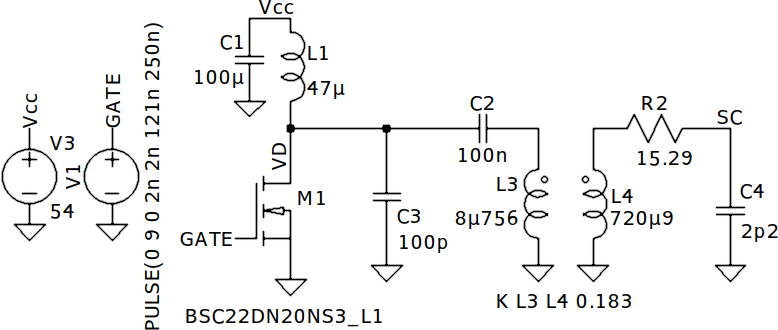
\includegraphics[width=\textwidth]{simon/resources/ltspice-complete.png}
    \caption{AAAAA}
    \label{fig:ltspice-complete}
\end{figure}



\section{The Interrupter}

\subsection{Fiber Optic Transmission}

% transmitter and receiver circuit

\subsection{MOSFET protection circuit}

Directly applying the interrupting technique to the class E circuit by just turning it on and off at any given moment would violate both the \gls{zvs} and \gls{zcs} conditions. In the worst case, switching the MOSFET on when the voltage is at its maximum and turning it off when the current is at its maximum a few thousand times a second would result in huge switching losses and device failure. Therefore a security mechanism has to be implemented.

One solution is to sample the interrupter signal and only apply it on every falling edge of the 4MHz base signal. The sampling could be done with a falling-edge triggered D-type flip-flop, whose output gets fed into an AND gate along with the base signal.

\begin{figure}[h!]
    \centering
    \caption{Bottom side text}
    \begin{circuitikz}[european]
      \draw (0,0) node[flipflop, flipflop def = {t1 = D, c3 = 1, n3 = 1, t3 = CLK, t6 = Q}](D){};
      \draw (4,.61) node[and port](A){};
      \draw (D.pin 6) -- (A.bin 1);
      \draw (D.pin 1) node[left]{INT};
      \draw (D.pin 3) ++(-.5,0) node[left]{4MHz} -- (D.pin 3);
      \draw (D.pin 3) ++(-.25,0) to[short, *-] ++(0,-.8) -- ++(3,0) node(n1){} -- (n1 |- A.bin 2) -- (A.bin 2);
      \draw (A.bout) ++(.4,0) node[right]{OUT};
    \end{circuitikz}
    \phantom{a}
    \vspace{10mm}
    \phantom{a}
    \begin{tikztimingtable}[timing/xunit = 5mm, timing/slope = 0.05]
      4MHz & 3{2{l}2{h}} N(a) 4{2{l}2{h}} N(b) 2{2{l}2{h}} \\
      INT  & 11{h} 16{l} 9{h} \\
      Q    & 12{h}16{l} 8{h} \\
      OUT  & 3{2{l}2{h}}16{l}2{2{l}2{h}} \\
      \extracode
      \draw[dotted, darkgray] (a) -- ++(0,-6);
      \draw[dotted, darkgray] (b) -- ++(0,-7);
    \end{tikztimingtable}
\end{figure}